\section{Response Calculation}
\label{chap:algorithms:response}
\subsection{Introduction}
In order to determine the spectroscopic response of an instrument (including
telescope and detector) spectrophotometric standard stars are observed
with the same setup as the science targets\footnote{For slit
  spectrrographs one generally uses a wide slit for flux standard
  stars to capture all flux.}. Spectrophotometric standard stars are
preferably observed during photometric conditions to reduce the
importance of atmospheric effects. After correcting for atmopsheric
effects the ratio between the reference spectrum of the standard star
and the observed spectrum will provide the response of the system.

If the science and/or standard star
data are observed during non-photometric conditions an absolute flux
calibration is impossible. For slit spectra the use of a narrow slit
introduces slit losses that are hard to correct. In many cases,
however, only a {\em relative} flux calibration is required, namely a
response curve that allows the user to correct the observed science
data for bumps and wriggles that were not corrected by the flat
fielding process.

The observed spectra of the standard
stars are first corrected for atmospheric effects:
\begin{enumerate}
\item The continuous {\em atmospheric extinction} is usually corrected
  with a standard extinction curve obtained for a given observatory,
  scaled with the airmass of the observation. During non-photometric
  conditions the actual extinction may be higher than the one
  tabulated in the extinction curve. The impact of this correction
  decreases with increasing wavelength. 
\item Wavelength above about 600\,nm\footnote{Ozone absorption affects
    the bluest part of ground-based data at about 310--330\,nm, but these are
    noticeable only in high S/N data.} are affected by {\em telluric
    absorption lines}. If these are not corrected the response curve
  will contain a mixture of instrument response and atmospheric
  response, especially if the reference spectra are free from telluirc
  lines (space-based data or model spectra). Reference spectra for
  many standard stars used for ESO instruments (e.g. UVES, FORS2,
  VIMOS) contain telluric lines
  (e.g. \cite{Hamuy+92,Hamuy+94}). For such reference spectra a
  telluric correction of the observed spectra is useless and one
  should instead interpolate the response across the regions of
  significant telluric absorption.
\end{enumerate}

Possibly the wavelength scale between the observed standard star
spectrum and the reference one needs to be aligned, either to correct
differences in radial velocity between the observed and the reference
spectrum in case of model spectra (e.g. X-shooter, SINFONI) and/or to
correct shifts introduced by imprecise positioning of the flux
standard star in the slit (e.g. VIMOS). If the differences in
wavelength become significant for a given resolution the division of
the reference spectrum by the observed one will create pseudo-P\,Cyg
prodiles, which will distort the response.

These requirements results in the algorithmic steps described in
Sect.\,\ref{response:main}.

\subsection{Testing}
Once the response determination has been implemented in HDRL and
incorporated in the SINFONI pipeline we tested it by calibrating one
standard star with the response curve from another (observed with the
same setup, but not necessarily during the same night). From the
resulting cube we extracted the one-dimensional spectrum with {\tt
  QFitsView} (using a radius of 11 pixels and {\tt sum}) and corrected
it with a background spectrum extracted with the same aperture. The
difference of the two spectra was then compared to the reference flux
for the standard star. Figures \ref{fig:Feige110_J},
\ref{fig:LTT7987_K}, and \ref{fig:Feige110_HK} show example
results. Due to the small number of observations only limited tests
were possible, which showed no problems that cannot be explained by
transparency differences between the observations of the standard stars.
 
\begin{figure}[H]
\centering \subfigure
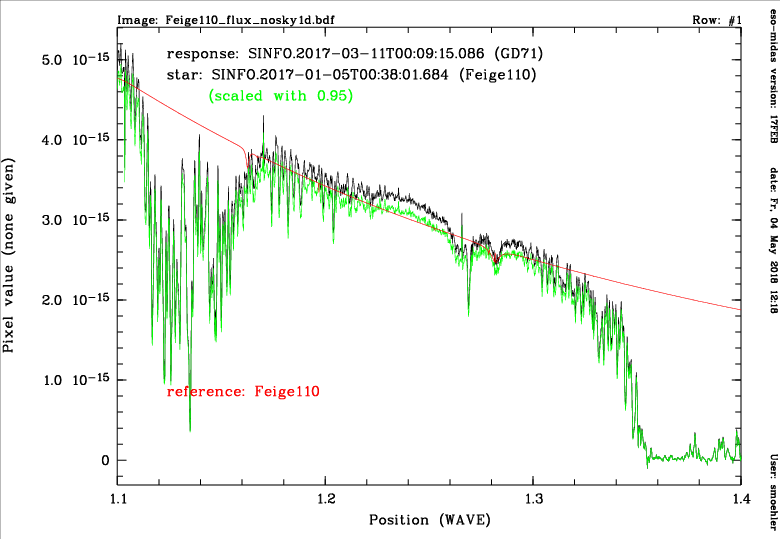
\includegraphics[width=16cm]{figures/Feige110_J.png} 
\caption[]
	{\footnotesize  The {\tt J} spectrum of the flux standard stars
          Feige\,110 calibrated with a response curve from the flux
          standard star GD\,71. The two stars were observed about 2
          months apart on nights of unknown quality. Scaling the
          flux-calibrated spectrum of Feige\,110 by 95\% achives good
          agreement with its reference data.}
	\label{fig:Feige110_J}
\end{figure}

\begin{figure}[H]
\centering \subfigure
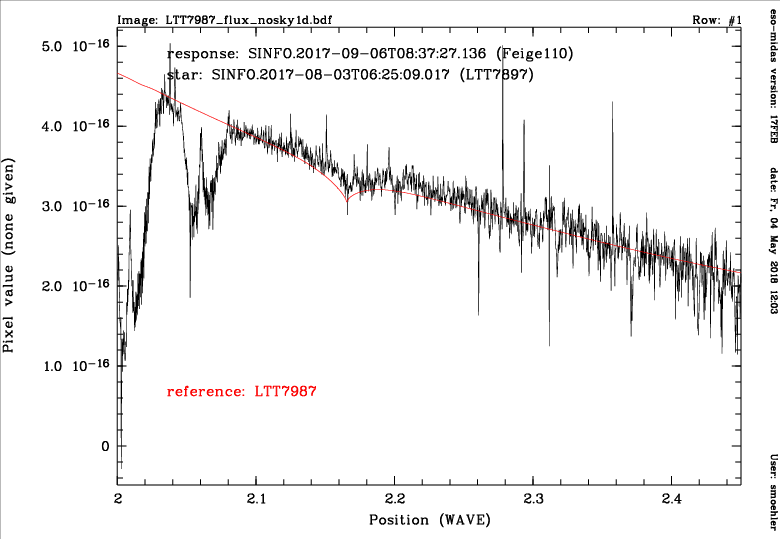
\includegraphics[width=16cm]{figures/LTT7987_K.png} 
\caption[]
	{\footnotesize  The {\tt K} spectrum of the flux standard stars
          LTT\,7987 calibrated with a response curve from the flux
          standard star LTT\,7987. The two stars were observed about 1
          month apart on nights of unknown quality. Nevertheless the
          flux-calibrated spectrum of LTT\,7987 agrees well with its
          reference data.} 
	\label{fig:LTT7987_K}
\end{figure}

\begin{figure}[H]
\centering \subfigure
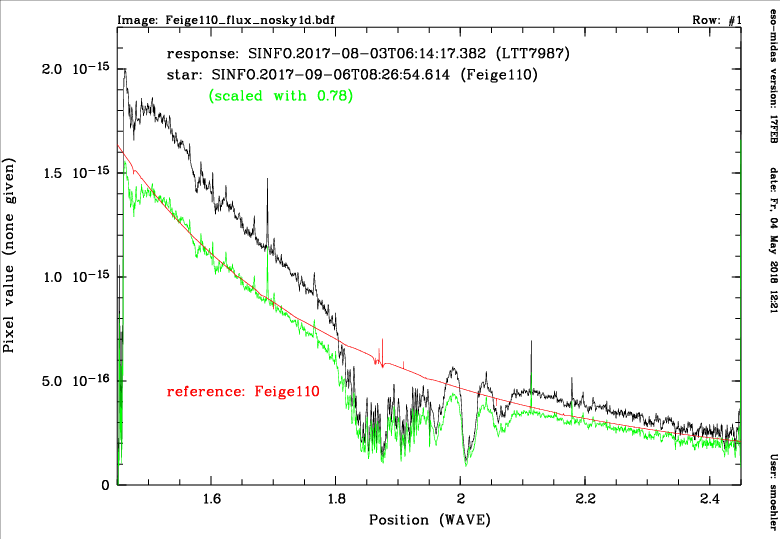
\includegraphics[width=16cm]{figures/Feige110_HK.png} 
\caption[]
	{\footnotesize  The {\tt H+K} spectrum of the flux standard stars
          Feige\,110 calibrated with a response curve from the flux
          standard star LTT\,7987. The two stars were observed about 1
          month apart on nights of unknown quality. Scaling the
          flux-calibrated spectrum of Feige\,110 by 78\% achives good
          agreement with its reference data.}
	\label{fig:Feige110_HK}
\end{figure}
